%% The following is a directive for TeXShop to indicate the main file
%%!TEX root = diss.tex

\chapter{Design}
\label{ch:Design}

%%%%%%%%%%%%%%%%%%%%%%%%%%%%%%%%%%%%%%%%%%%%%%%%%%%%%%%%%%%%%%%%%%%%%%
%%
%% Naive Implementation
%%
%%%%%%%%%%%%%%%%%%%%%%%%%%%%%%%%%%%%%%%%%%%%%%%%%%%%%%%%%%%%%%%%%%%%%%
\section{Straightforward Implementation}
\label{sec:Straightforward Implementation}
In this section we propose an implementation of a cache that combines inter-line and intra-line compression techniques. This implementation is built simply by combining \hyperref[sec:Dedup]{Dedup} and \hyperref[sec:BDI]{BDI}. This cache is thus able to perform deduplication on BDI compressed blocks and uses the same infrastructure and a similar replacement policy to \hyperref[sec:Dedup]{Dedup}.

\subsection{Structure}
\label{ssec:DedupBDIStructure}
\begin{figure}
    \makebox[\textwidth][c]{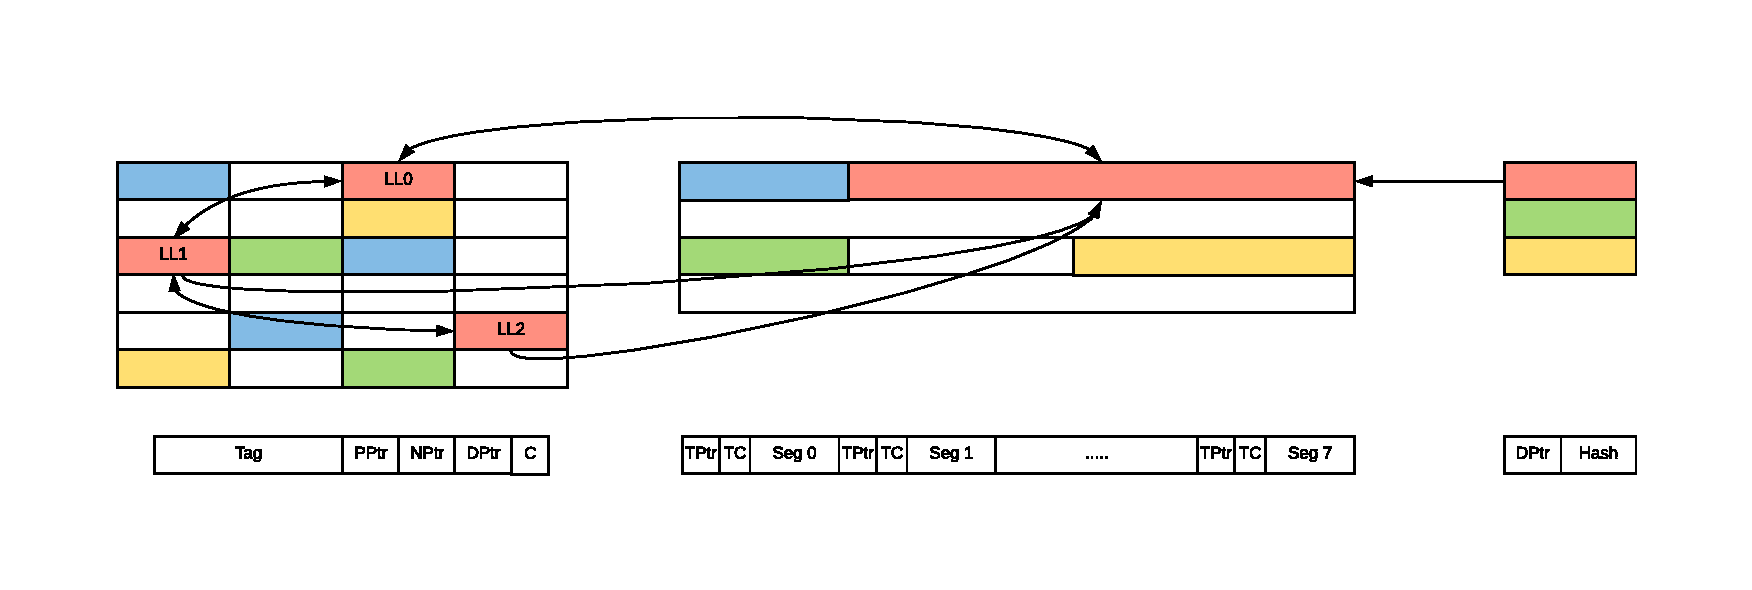
\includegraphics[width=1.5\textwidth]{DedupBDI.pdf}}
    \caption[DedupBDI Cache]{From top to bottom: Conventional, BDI, Dedup, DedupBDI. showing one set from the data array of each, and one or more sets from the tag array.}
    \label{fig:DedupBDI}
\end{figure}
The cache consists of three arrays: a tag array, a data array, and a hash array. Unlike a normal cache and similar to a \hyperref[sec:Dedup]{Dedup} cache, the tag and data arrays are decoupled and do not have a one to one mapping. Instead, related tags and data entries have to be able to point to each other.\par
On top of it's normal operation, the tag array is also used to save compression and deduplication metadata. The hash array is needed to facilitate searching for similar data lines to enable deduplication.\par
The general structure of the cache is shown in Figure \ref{fig:DedupBDI}.
\subsubsection{Tag Array}
\label{sssec:DedupBDITag}
\begin{figure}
    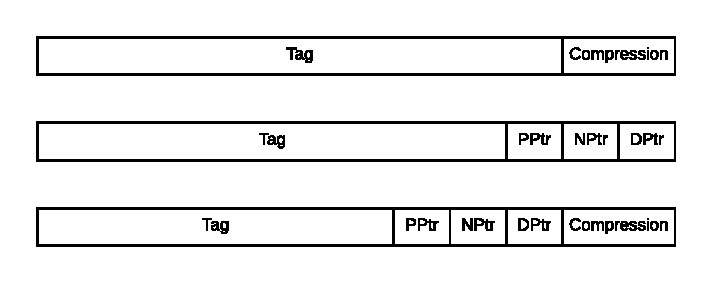
\includegraphics[width=\textwidth]{BDIvsDedupvsDedupBDI_Tag.pdf}
    \caption[DedupBDI Tag Array]{From top to bottom: the figure shows three tag entries and their metadata from the BDI, Dedup, and DedupBDI Caches.}
    \label{fig:DedupBDI_Tag}
\end{figure}
The DedupBDI tag array is a normal, set associative array with no limitations on its associativity or organization. It incorporates extra features from \hyperref[sssec:DedupTag]{Dedup} and \hyperref[sssec:BDITag]{BDI} to support dealing with deduplicated and compressed data lines.\par
Deduplication in its essence means that multiple tags that have similar data lines will be allowed to only save one copy of this data. This breaks the conventional one to one relationship between tags and data in a normal cache making the tag and data caches decoupled. Because of this, a tag entry needs an extra pointer to its corresponding data entry. Unlike \hyperref[sssec:DedupTag]{Dedup tag array}'s data pointer, this pointer needs to be able to point to compressed data lines that are smaller in size than normal cache lines. The pointer essentially needs to be larger in size to be able to address lines of smaller granularity. It is actually divided into two pointers: a data set pointer, and a segment pointer, allowing the tag to point to a compressed line anywhere withing the data array boundaries.\par
Similar to \hyperref[sssec:BDITag]{BDI}, The tag entries also need to save compression encoding to be able to resolve the size of the compressed data it points to.\par
Similarly to \hyperref[sssec:DedupTag]{Dedup}, tag entries that share the same deduplicated data line are arranged in a linked list, facilitating their eviction in case that data line is evicted. So each tag entry has two extra previous/next pointers to allow them to form a linked list. Those pointers need to be big enough to point to tag sets. Since reading a tag requires reading the whole set, the required tag from that set can be resolved by comparing it's data pointer. The use of a linked list is necessary in case of data line eviction.\par
In general, the tag array must have more tag entries than the data array, otherwise it wouldn't be able to utilize compression and deduplication. The structure, metadata, and differences between tag entries in Dedup, BDI, and DedupBDI is shown in Figure \ref{fig:DedupBDI_Tag}. It shows previous and next pointers in Dedup and DedupBDI tags, segment pointers in BDI, and data pointers in Dedup and DedupBDI.
\subsubsection{Data Array}
\label{sssec:DedupBDIData}
\begin{figure}
    \makebox[\textwidth][c]{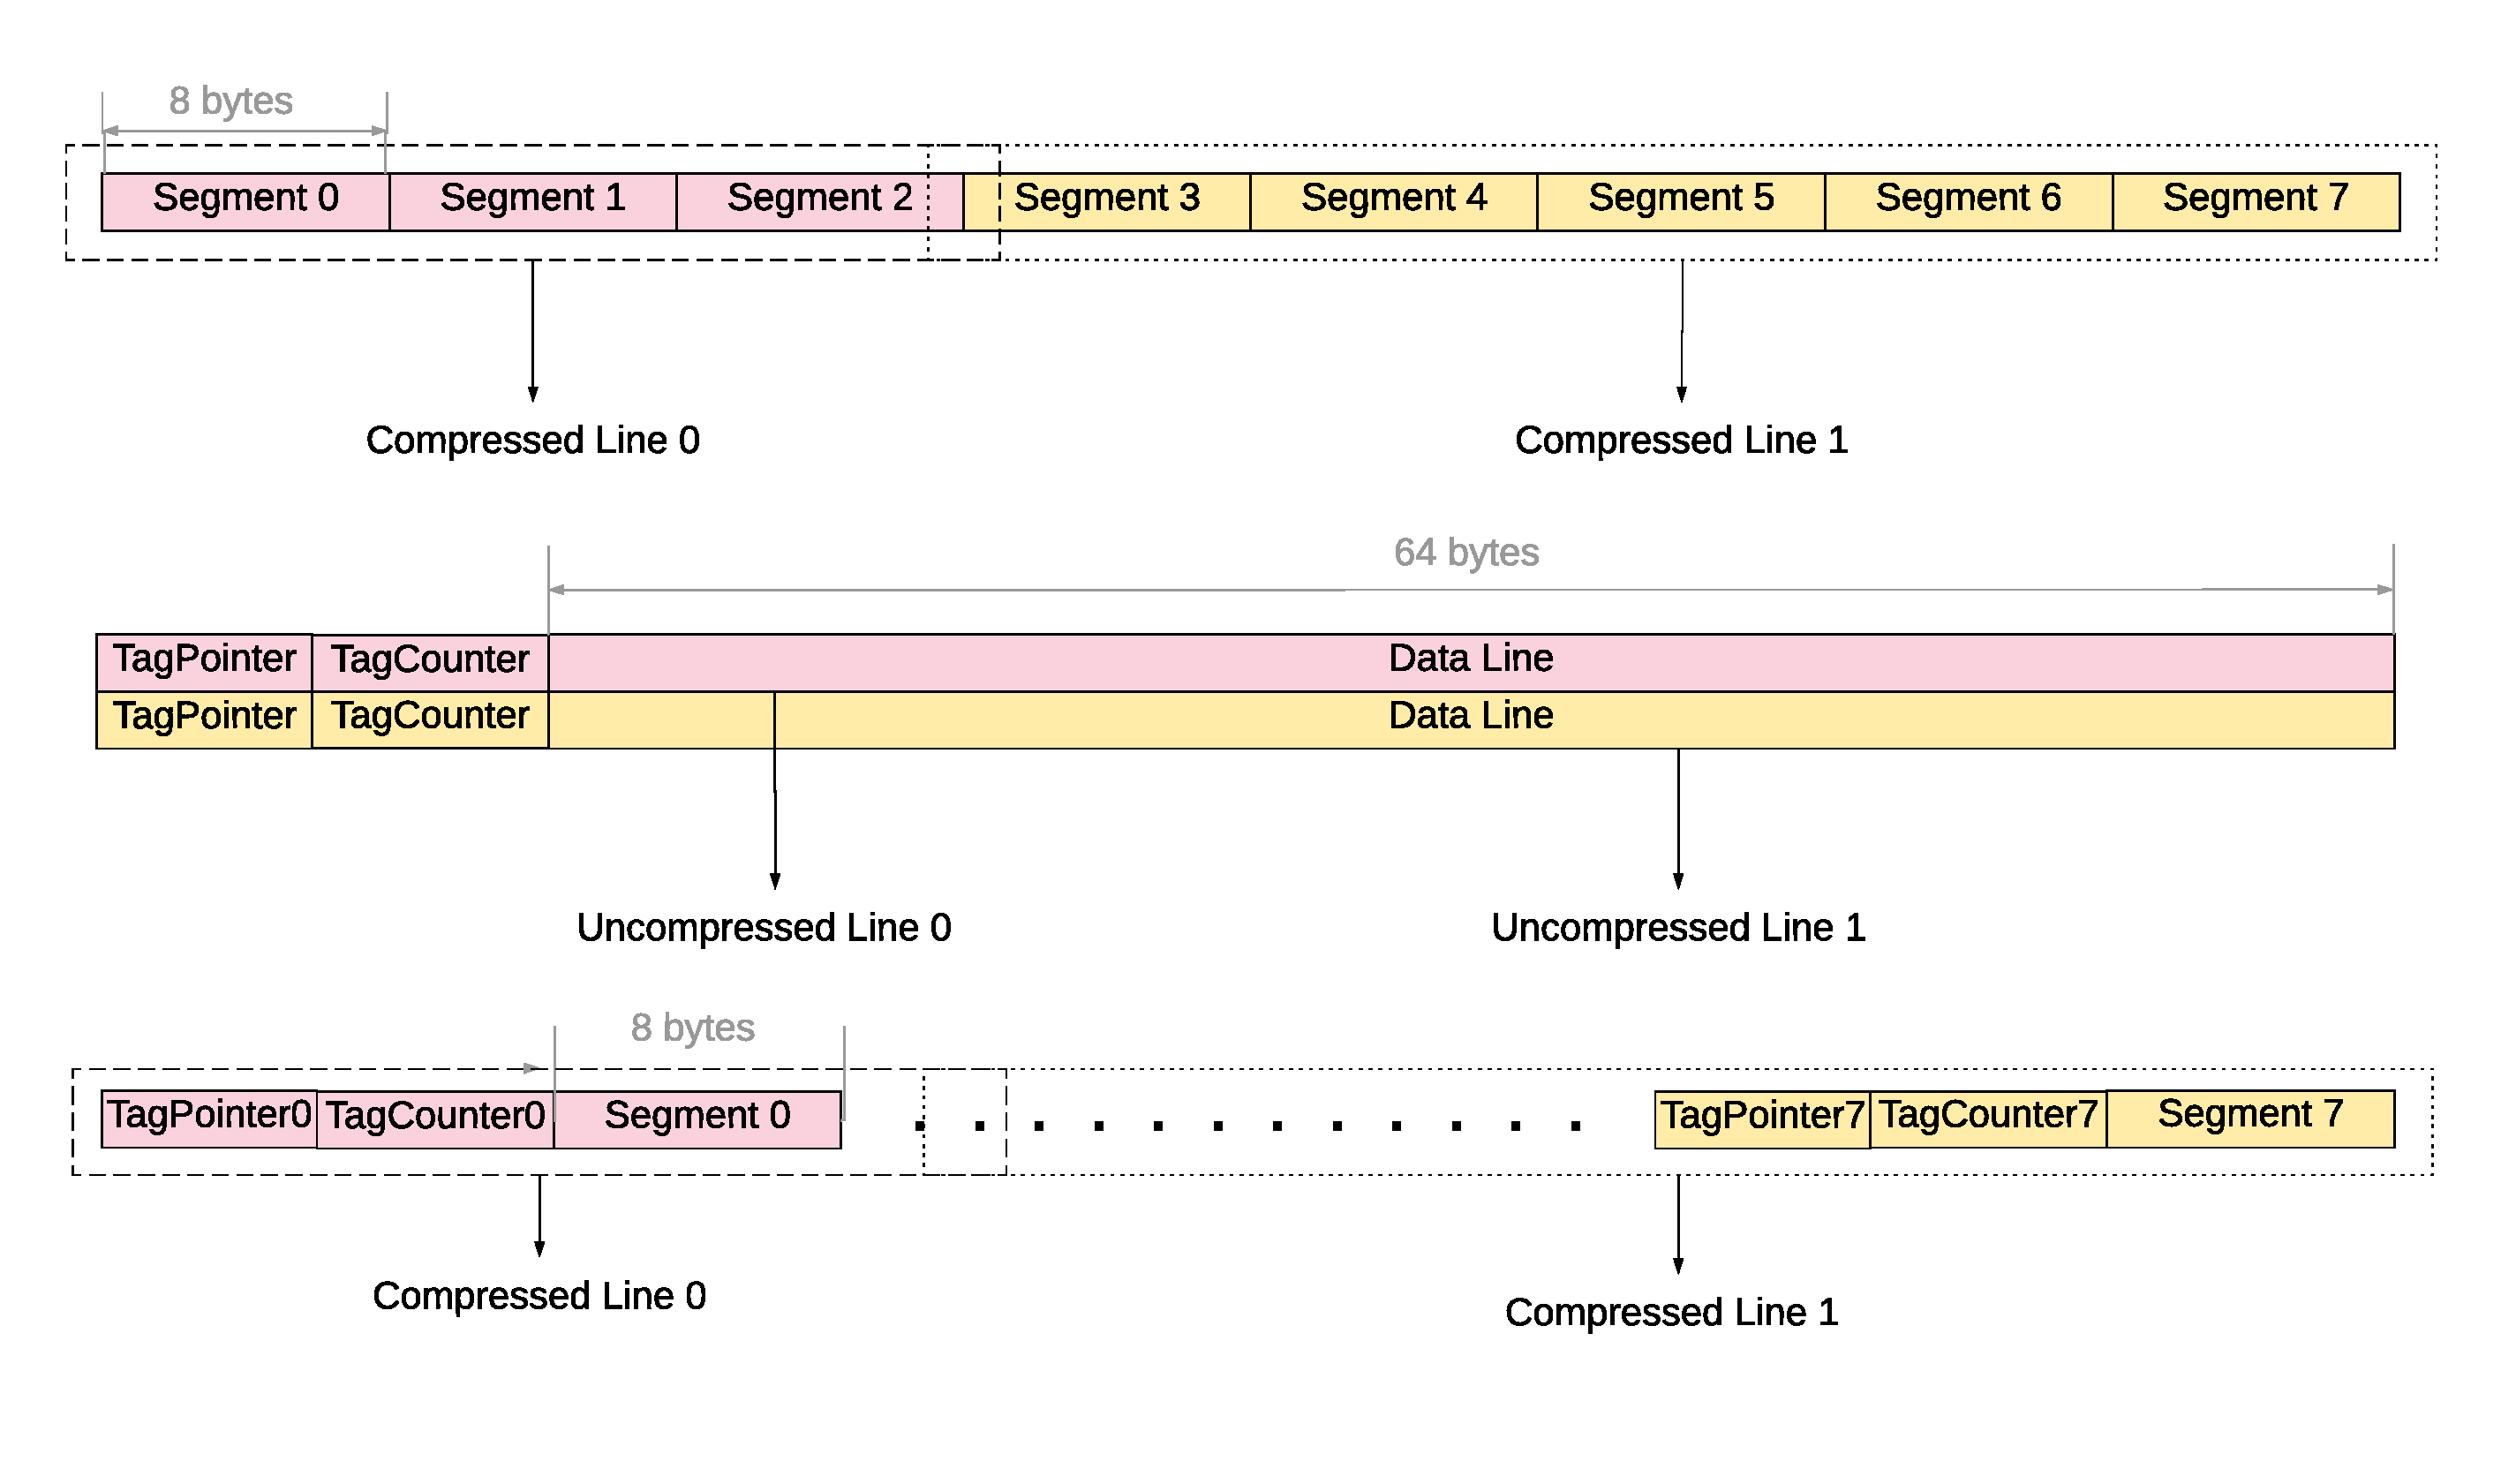
\includegraphics[width=1.5\textwidth]{BDIvsDedupvsDedupBDI_Data.pdf}}
    \caption[DedupBDI Data Array]{From top to bottom: the figure shows three data entries and their metadata from the BDI, Dedup, and DedupBDI Caches.}
    \label{fig:DedupBDI_Data}
\end{figure}
The DedupBDI data array is similar to that of a \hyperref[sssec:BDIData]{BDI} cache, each data line in the DedupBDI data array is logically divided into eight segments of eight bytes each (assuming a 64 byte cache line). A compressed data line can occupy any number of segments between one and eight, in the best case scenario all lines will be compressed into one segment each.\par
The data array is decoupled from the tag array because it must also support deduplication. In case a compressed data line is evicted, all the tags associated with it must also be evicted. The compressed data line then must be able to point to the tag linked list and to know how long that list is. Accounting for the best case scenario where each line is compressed into one segment, each segment must have two metadata fields: a pointer to the head of the tag linked list that's associated with this line, and a counter of the tags in that linked list. Both those fields are useful in case an eviction of a data line happens.\par
The pointer needs to be big enough to only point to a tag set. The target tag from this set can be known by comparing its data pointer. The counter only needs to be two bits large, as it represents zero/one/two/more. In cases of eviction it can be determined if the count is less than 3 by checking only one tag entry for previous and next pointers.\par
The structure and difference between tag entries in Dedup, BDI, and DedupBDI is shown in Figure \ref{fig:DedupBDI_Data}
\subsubsection{Hash Array}
\label{sssec:DedupBDIHash}
The hash array is a simple set associative structure. It's used to store hashes of some of the data lines providing a way to facilitate finding similar lines and deduplicate them. It is the same as that of a \hyperref[sssec:DedupHash]{Dedup} cache. When a data line is hashed the hash is split into two parts: one is used to index the hash array, while the other is saved in the hash array itself, similar to the tag part of the address being saved in data array.\par
With each entry in the hash array there's also a pointer to a data line that meets this hash. Just like the data pointers in the tag array, the pointer is actually two parts: one points to the data set, and the other to the segment in that set.\par
The hash itself is computed like \hyperref[sssec:DedupHash]{Dedup}, through an XOR tree. Based on experiments done in \cite{dedup} this is enough to keep hash collisions less than 1%.

\subsection{Operations}
\label{ssec:DedupBDIOperations}
\subsubsection{Cache Read}
\begin{figure}
    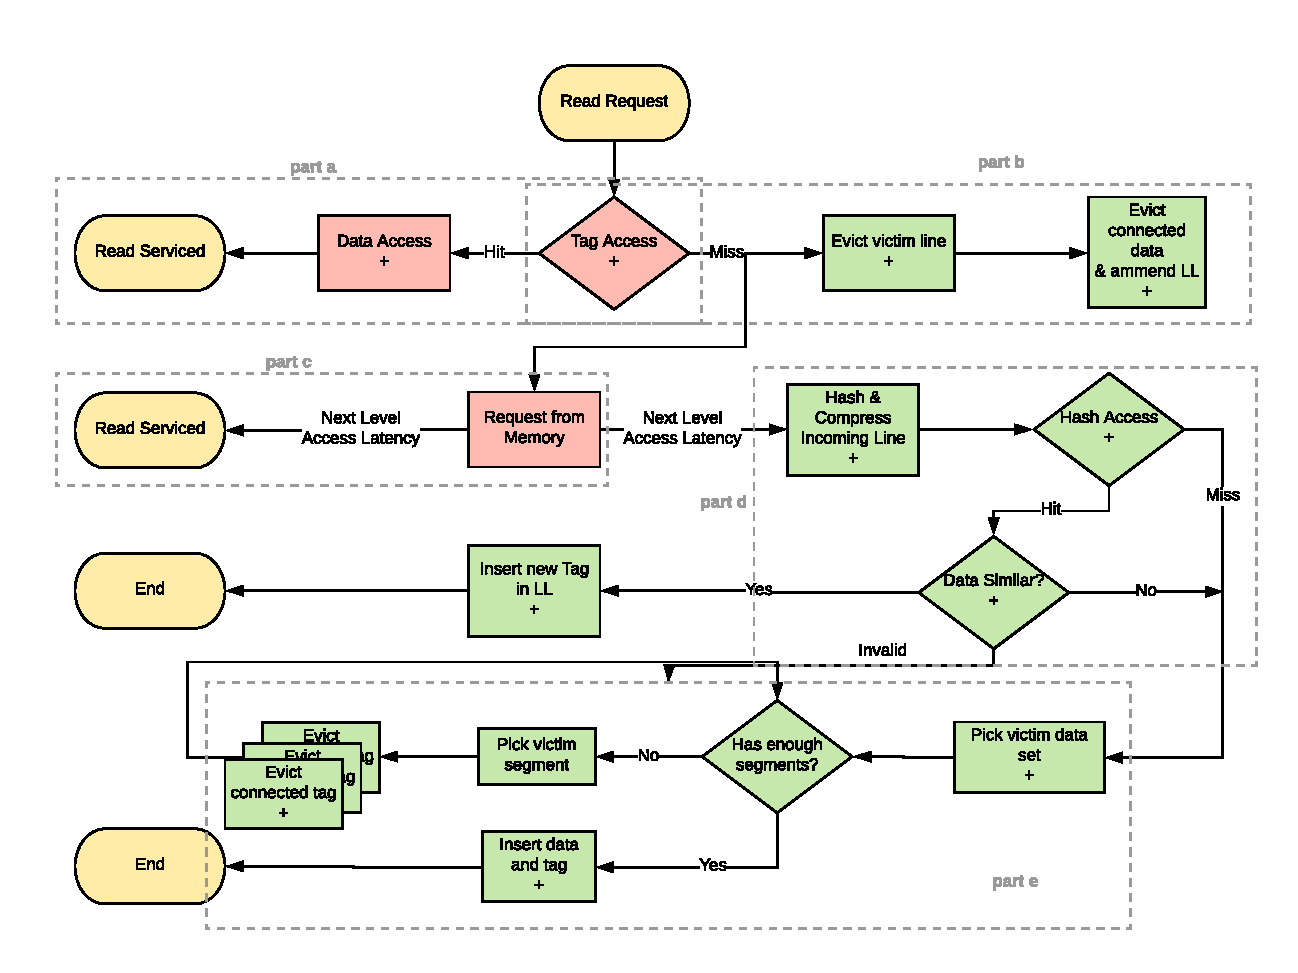
\includegraphics[width=\textwidth]{DedupBDI_Read.pdf}
    \caption[DedupBDI Read]{The flowchart shows the sequence of actions triggered by a read access to the DedupBDI cache. Red blocks signify actions happening on the critical path, while green blocks mean actions happening off the critical path. Each + sign in any of the blocks signifies an extra latency for tag array access, data array access, or compression.}
    \label{fig:DedupBDI_Read}
\end{figure}
A flowchart for the Dedup cache read is shown in Figure \ref{fig:DedupBDI_Read}. When the request first arrives the tag array is accessed. Part a in the figure shows the case when the tag access results in a hit, and the tag points exactly to the required line, then the data line can be read, decompressed, and sent back to the requester right away. If the tag access is a miss, as shown in part b, the victim line is evicted. If the tag was connected to a distinct data line it is deleted as well, otherwise the linked list containing the tag has to be updated. Updating the linked list in this case means changing the pointers of the previous and next elements to point to each other instead of the victim.\par
Then at the same time in parallel, a request is sent to the next cache level (or main memory). Once the requested line comes back from the next level it can be used to service the requester right away, as shown in part c. Inserting the line itself into the cache happens after that and off the critical path.\par
Other than updating the linked list if needed, everything in the access so far is similar to a conventional cache. The insertion of the new line is going to be different. The insertion of the new line starts in part d in the figure. Once the requested line comes back from next level, and in parallel to serving the requester, the line is hashed and compressed. Then the hash is used to access the hash array.\par
If the hash access hits, then the incoming line must be compared to the line pointed to by the hash, to make sure there are not collisions. There are four outcomes of this scenario, shown in part d:
\begin{itemize}
    \item \textbf{Hash Miss:} No similar hash is found, either because similar lines do not exist in the data array, or because the hash array is not big enough to keep track of all data lines. In this case we use the data replacement policy to pick a set and evict compressed data line(s) until a sufficient area for the compressed line exists. The new tag is inserted and the tag and data lines have to point to each other, the tag will not point to other tags and will not create a linked list because no deduplication is happening yet. A new hash entry will be selected based on the hash replacement policy and will point to the newly inserted data line. This is shown in part e of the figure.
    \item \textbf{Hash Hit, Line Similar:} In which case the received data line can be deduplicated. It will use the same data line and hash entry. Only the new tag needs to be inserted. It is inserted as the head of the linked list and points to the deduplicated data line. The data line's tag counter (deduplication counter) has to be incremented and it has to point to the new linked list head.
    \item \textbf{Hash Hit, Line Invalid:} Because hashes point to data lines, but data lines do not point to hashes, when a data line is evicted, it's associated hash might not, causing a situation like this to arise.\par
        In this case, we utilize the invalid space right away instead of consulting the data replacement policy. This is similar to the same case in \hyperref[ssec:DedupOperations]{Dedup} with one minor difference: if the invalid space is not enough for the compressed line, we use the data replacement policy to start evicting from the current data set until a sufficient area is enough for the compressed data line to be inserted.\par
        The tag entry is also inserted. It has to point to the data line, but it doesn't point to any other tags because the data line is not deduplicated yet and shouldn't have a linked list associated with it. The data line in return also has to point to the tag entry, the hash entry is not changed because it already points to the space we used for the data line. This case is also shown in part e.
    \item \textbf{Hash Hit, Line Different:} This case happens only on a hash collision. Once a collision happens, it's treated like a hash miss with one modification. A new hash insertion is not needed, the same hash entry will be changed to point to the newly inserted data line in only if the line it was previously pointing to was not deduplicated (i.e. Its tag counter is 1). Otherwise it remains untouched. This follows the same policy used in \hyperref[ssec:DedupOperations]{Dedup}.
\end{itemize}
To avoid segmentation, the authors assume compaction always happens in the data array before each insertion, this is in accordance with previous work.
\subsubsection{Cache Write}
\begin{figure}
    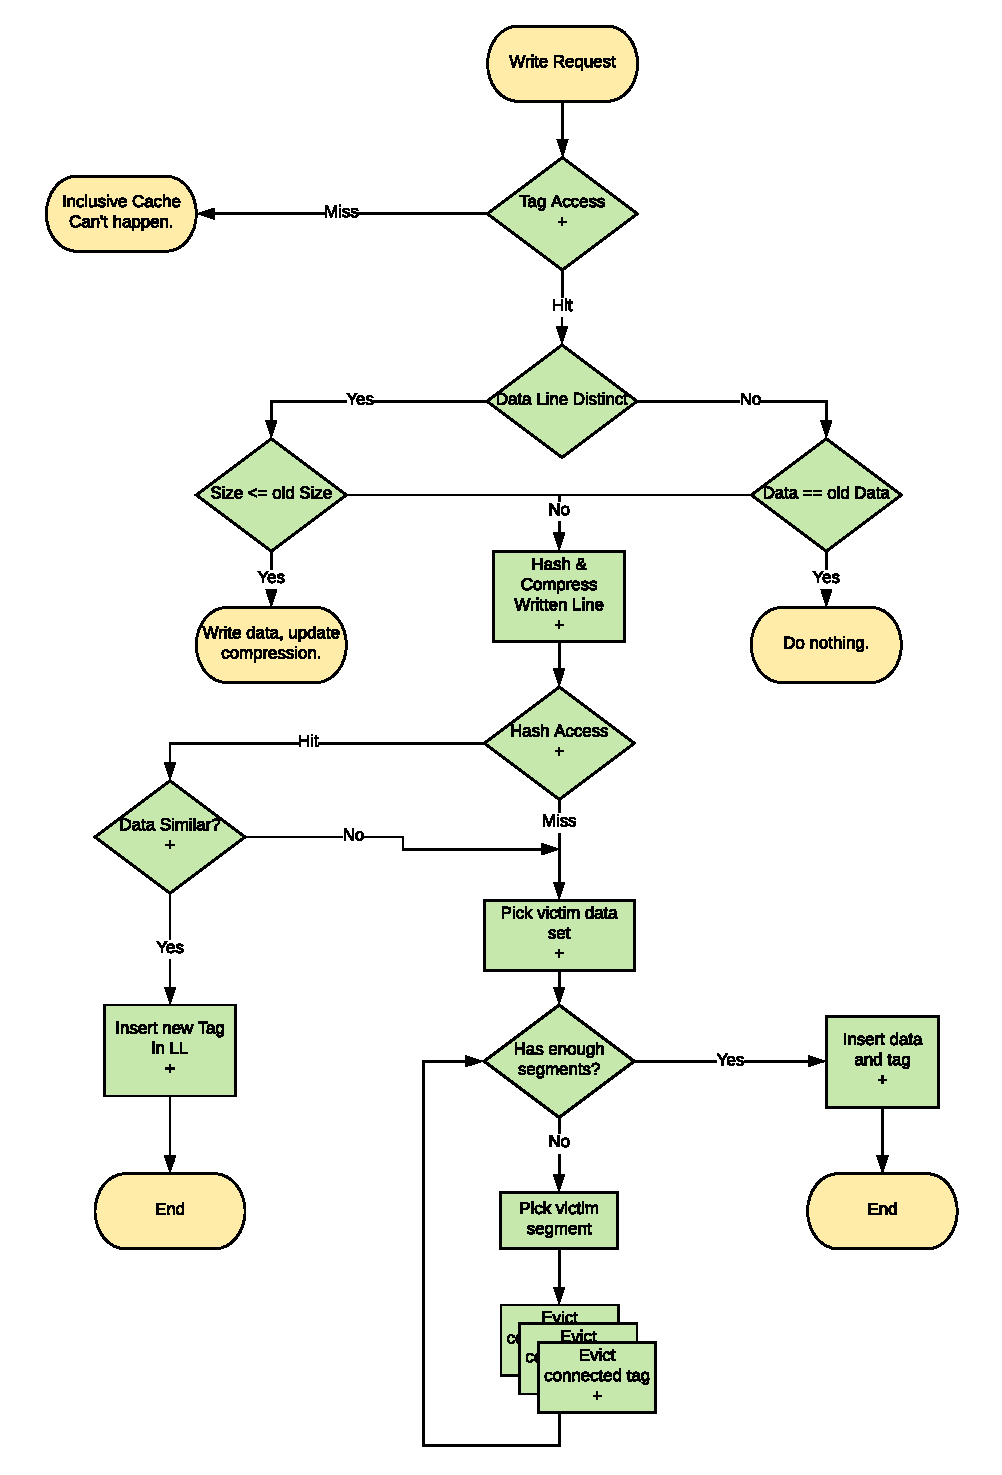
\includegraphics[width=\textwidth]{DedupBDI_Write.pdf}
    \caption[DedupBDI Write]{The flowchart shows the sequence of actions triggered by a write access to the DedupBDI cache. All the blocks are shaded in green because any write request should be off the critical path of the processor regardless of its status in the cache (hit or miss). Each + sign in any of the blocks signifies an extra latency for tag array access, data array access, or compression.}
    \label{fig:DedupBDI_Write}
\end{figure}
A flowchart of write access to a DedupBDI cache is shown in Figure \ref{fig:DedupBDI_Write}. Because we always use inclusive caches, if a line is in a lower level cache it must also be in it's parent. A cache miss on a write request thus can never happen and a tag array access on a write request will always yield a hit as shown in part a. In parallel to the tag access, the written data line can also be hashed.\par
Once the tag access is finished, we can find out whether the line was distinct or not. If the line had no other tags associated with it and the new size is less than or equal to the original size, then it can be written to right away as shown in part b. If the line is deduplicated, then a write to the line can change it and cause that tag to lose similarity. The insertion of the written data line then can be handled similarly to a miss. It has to access the hash array and look for similar lines, this has one of the four outcomes described above as shown in parts c and d.

\subsection{Replacement Policies}
\label{ssec:Replacement Policies}
Some parts of the DedupBDI cache like the tag array can still operate in the same way with the same replacement policies. The tag array can use one of the known replacement policies like LRU. Other parts of the cache have to be treated differently. Since the data and hash array are decoupled from the tag array each one of them needs it's own replacement policy.
\subsubsection{Data Array}
\label{sssec:DedupBDIDataRepl}
The data array uses a somewhat similar replacement policy to \hyperref[sssec:DedupDataRepl]{Dedup data replacement policy}. A free list keeping track of free data sets (not lines) is used, whenever needed an entry of this list was used to insert a line. If the list if empty then up to four data sets are picked at random, if any of the sets have enough segments for insertion of the line then it's selected right away, otherwise the one with the least sum of deduplication counters is picked.\par
The picked data set then is used for the second part of the replacement policy, in which a segment (or group of segments representing a compressed data line) with the lowest deduplication counter is selected for eviction. Segments keep evicted as necessary until a large enough space is freed for the insertion. Each segment or group of segments evicted can trigger a chain of evictions for the tag linked list associated with it.
\subsubsection{Hash Array}
\label{sssec:DedupBDIHashRepl}
The hash array is indexed by a part of the hash, the selection of a victim hash set is thus dependant on the hash that needs to be inserted. Once that set is selected, a hash entry is then selected based on the number of deduplications on the data line it point to. If this data line is not deduplicated then this hash can be used and overwritten. Otherwise it's not touched. The rationale behind this is to keep hashes pointing to deduplciated lines from getting evicted and causing the cache to miss extra deduplication for a newly incoming line that might not be useful for deduplication.

%%%%%%%%%%%%%%%%%%%%%%%%%%%%%%%%%%%%%%%%%%%%%%%%%%%%%%%%%%%%%%%%%%%%%%
%%
%% Upper Bound
%%
%%%%%%%%%%%%%%%%%%%%%%%%%%%%%%%%%%%%%%%%%%%%%%%%%%%%%%%%%%%%%%%%%%%%%%
%% TODO: should we discuss "How did we decide what to idealize?". I think we
%% should have a results section for each implementation, to motivate the
%% section after it!
\section{Establishing an Upper Bound}
\label{sec:Upper Bound}
To be able to evaluate the straightforward design we discussed in the previous section, an upper bound must be established. We try to get the upper bound of enhancements by idealizing the design choices we have selected. There are two aspects we can idealize in this design:
\begin{itemize}
    %TODO: Dump data lines, show missed dedup and quantify.
    \item \textbf{Finding a similar line:} Finding a similar line in the DedupBDI cache has two sources of possible error: The first is the hashing itself. Because hashing data lines to a smaller space means it will never be perfect and collisions are inevitable. The second limitation is the size of hash array. Because the number of entries in the hash array is less than that of the data array, there's a chance that an opportunity for deduplication is missed because the hash array was too small and couldn't keep its hash. Finding a similar line can be idealized by directly searching through the data array and comparing each line until a similar data line is found.
    %TODO: Show figure of data utilization here.
    %TODO: Show L2 Back Invs and use NMRU as ideal instead of LRU?
    \item \textbf{Replacement of data lines:} Imperfections in the replacement policy of data array comes from two sources: the first is the free list, since we cannot make the free list keep track of all free segments in the data array because it would be impractically large, it can only keep track of free sets, that means even if only one segment is used from a set that set is not kept in the free list anymore. The second source is the random selection of data lines whenever the free list is empty, our experiments showed that the random selection causes utilization of the data array to always be less than a 100\% as shown in \ref{ch:Results}, selecting 4 random sets might not always yield a set with enough free segments, selecting more than 4 can be time inefficient. We idealize the replacement policy by directly searching the whole data cache for free segments that are enough to insert a new compressed line, this ensures a 100\% utilization of the data array, if no free segments are available we use data array wide LRU to pick a victim segment(s) instead of doing it randomly.
\end{itemize}
with the use of perfect deduplication and data insertion, a hash array is no longer needed, and the tag array is no different than a normal cache. The \ref{ch:Results} chapter shows the performance of both the straightforward implementation and the idealized one.



%%%%%%%%%%%%%%%%%%%%%%%%%%%%%%%%%%%%%%%%%%%%%%%%%%%%%%%%%%%%%%%%%%%%%%
%%
%% Final Implementation
%%
%%%%%%%%%%%%%%%%%%%%%%%%%%%%%%%%%%%%%%%%%%%%%%%%%%%%%%%%%%%%%%%%%%%%%%
\section{Final Implementation}
\label{sec:Final Implementation}
In order to improve on the naive implementation and towards the upper bound, we propose the following realistic improvements on the straightforward implementation.
\begin{itemize}
    %TODO: Quantify this
    \item \textbf{Deduplication:} while any realistic deduplication will still depend on the existence of a hash array. The hash array used in the straightforward was the same as \hyperref[sssec:DedupHash]{Dedup}, the hash array was enough to cover deduplications in the data array of \ref{sec:Dedup}, but because of the use of compression in DedupBDI, each line can hold up to eight times the amount of data, the same hash array with the same number of entries might not be enough to cover that amount of deduplication efficiently. In the \ref{ch:Results} we show how varying the number of hash array entries can affect the performance of deduplication in DedupBDI cache.
    \item \textbf{Data free list:} To keep track of all free segments in the data array, a modification to the free list was made, the free list is now divided into multiple free lists, each of which can keep track of data sets with a certain amount of free segments. Namely we have eight free lists: the first keeps track of data sets with one free segment and the second with two, until the last which keeps track of data sets with eight or more free segments. Whenever a data line needs to be inserted, the free list corresponding to its size is looked up first. If it's empty then the larger ones are searched one by one. If no empty segments exist then we return to the second part of the replacement policy.
    %TODO: Results of L2 back invs.
    %TODO: Need to quantify LRU vs Rand vs NMRU
    %TODO: Quantify how it hurts
    \item \textbf{Replacement of data lines:} Two modifications of the replacement policy were introduced. The first is ignoring the replacement policy in case of a tag miss, hash hit, but invalid data line was found to be hurting the performance as in some cases the space of the invalid line might not be enough but another enough space might exist, the better alternative is to always consult the replacement policy. The second change I cannot write about until I quantify.
\end{itemize}
